% ChapterPub1
\label{ChapterPub1}




%\lhead{Chapter 2. \emph{Methods}} % This is for the header on each page - perhaps a shortened title

%\pagestyle{empty}

%\setcounter{chapter}{0}
\chapter{Manuscript}
%\addcontentsline{toc}{chapter}{Wolfisberg \textit{et al.}, Journal of Virology, Submitted November 2015}  
\begin{center}
\addtocontents{toc}{\cftpagenumbersoff{chapter}}
\vspace{5.5cm}

\LARGE{\textbf{Late maturation steps in the nucleus preceding pre-lytic active egress of
progeny parvovirus.}}

\vspace{3cm}

Raphael Wolfisberg, Christoph Kempf and Carlos Ros
\end{center}


\afterpage{\blankpage}
\phantomsection\addcontentsline{toc}{section}{Late Maturation Steps in the Nucleus Preceding Pre-Lytic Active Egress of Progeny Parvovirus.}



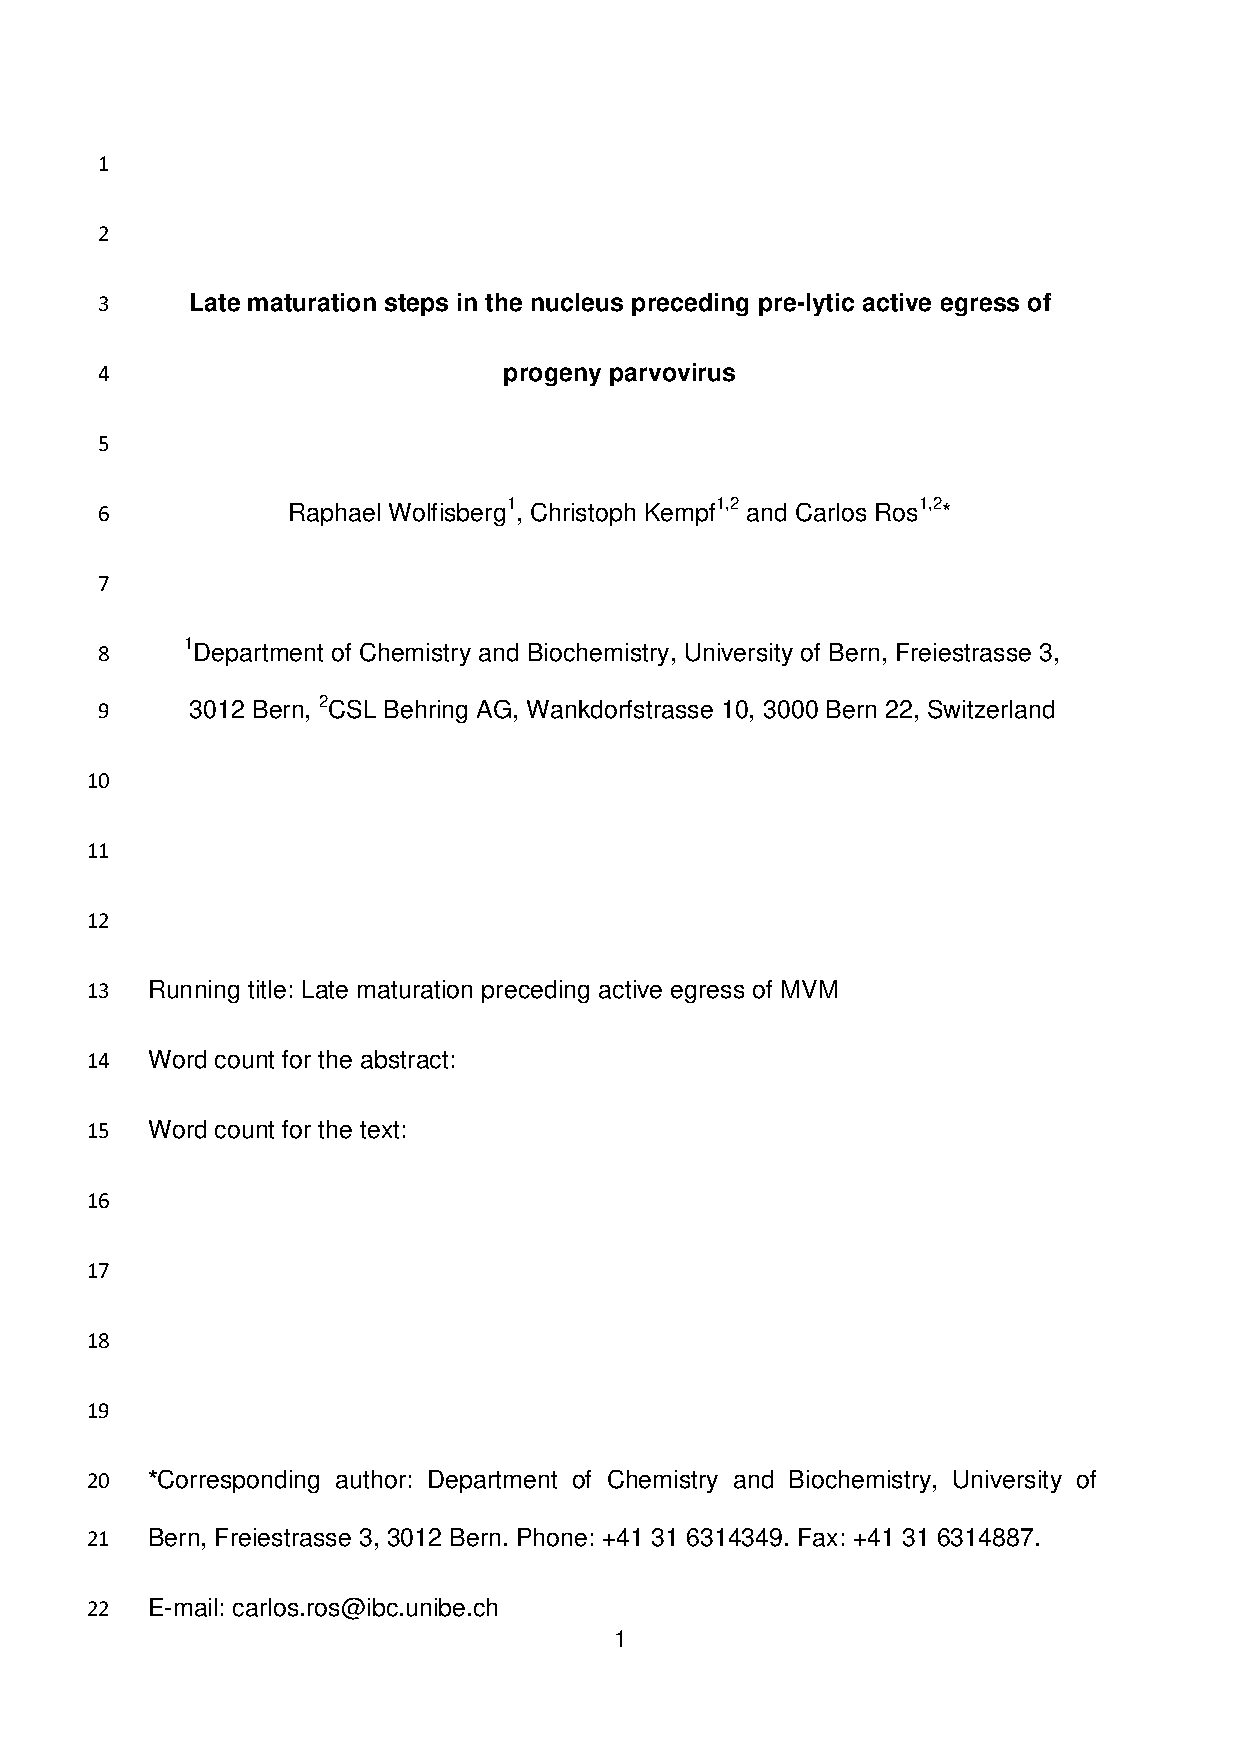
\includepdf[pagecommand=\thispagestyle{empty}, pages={1-34}, offset=5 0, scale=1]{../pdfdocuments/Manuscript}
\includepdf[pagecommand=\thispagestyle{empty}, pages={1-8}, offset=5 0, scale=1]{../pdfdocuments/Figures}
\label{ChapterPub1End}

